% !TeX spellcheck = fr_FR
\chapter{Les \Jiben{} \Jianfa{}}\label{ch:jibenjianfa}

Le terme  \Jiben{} \Jianfa{} (\begin{CJK*}{UTF8}{bsmi}基本劍法\end{CJK*}) désigne ce qu'on appelle généralement les techniques de base de l'épée. On peut le traduire mot à mot par : les \textit{méthodes} (\Fa{}) \textit{basiques}, \textit{élémentaires}, \textit{fondamentales} (\Jiben{}) de l'\textit{épée droite} (\Jian{}).

Les différents styles de \Taijijian{} présentent un nombre variable de \Jiben{} \Jianfa{}, habituellement entre quatre et treize ou même plus. On trouve déjà le nom de plusieurs de ces techniques dans le \JianJing{}, un traité d'épée écrit par \YuDayou{} aux environs de 1560, ou dans le \WubeiZhi{}, une encyclopédie militaire qui aurait été publiée en 1620.
Il n'est pas certain cependant que ces termes se rapportaient déjà aux techniques qu'ils décrivent aujourd'hui en \Taijijian{}, d'autant moins que les noms des \Jiben{} \Jianfa{} sont loin de toujours se correspondre d'un style à l'autre.

La tradition du \Yangjia{} \Michuan{} \Taijijian{} énumère huit \Jiben{} \Jianfa{}, chacun correspondant à une des huit sections de la forme d'épée \Kunlun{} : \Pi{}, \Ci{}, \Liao{}, \Zha{}, \Mo{}, \Duo{}, \Tiao{}, \Hua{}.
Un neuvième, \Dian{}, est aussi mentionné mais est parfois décrit comme la combinaison de \Pi{} et \Ci{}, peut-être pour préserver le nombre parfait de huit techniques pures.
Quelle qu'en soit la raison, j'ai le sentiment que cette description de \Dian{} en tant que combinaison, constitue un aveu de la possibilité d'associer les \Jiben{} \Jianfa{} entre eux.
Je préfère donc les considérer, non pas comme des techniques en soi, mais plutôt comme des principes techniques qu'on peut combiner pour générer l'ensemble des techniques possibles. Ce qu'on appelle alors \textit{techniques de base} seraient ainsi simplement les techniques représentatives des \Jiben{} \Jianfa{} qui les constituent.

L'examen des caractères chinois pour les huit \Jianfa{} du \Yangjia{} \Michuan{}, révèle que quatre d'entre eux (\Pi{} \begin{CJK*}{UTF8}{bsmi}劈\end{CJK*}, \Ci{} \begin{CJK*}{UTF8}{bsmi}刺\end{CJK*}, \Duo{} \begin{CJK*}{UTF8}{bsmi}剁\end{CJK*}, \Hua{} \begin{CJK*}{UTF8}{bsmi}劃\end{CJK*}) possèdent la clé graphique du couteau, tandis que les autres (\Liao{} \begin{CJK*}{UTF8}{bsmi}撩\end{CJK*}, \Zha{} \begin{CJK*}{UTF8}{bsmi}扎\end{CJK*}, \Mo{} \begin{CJK*}{UTF8}{bsmi}抹\end{CJK*}, \Tiao{} \begin{CJK*}{UTF8}{bsmi}挑\end{CJK*}) contiennent la clé de la main. On peut donc avancer que les quatre premiers précisent principalement la manière dont la lame est utilisée pour couper ou percer tandis que les autres décrivent plutôt le mouvement général (soulever, fouetter, etc.) indépendamment de l'arme. On trouve par exemple les caractères \Liao{} et \Zha{} dans le nom de techniques de lance, de bâton ou même de boxe, citées dans divers manuels d'arts martiaux historiques. La neuvième technique, \Dian{} \begin{CJK*}{UTF8}{bsmi}點\end{CJK*}, dont le nom signifie \textit{pointer}, est encore une exception puisqu'elle ne contient aucune des deux clés graphiques et ainsi, mettrait l'accent sur l'utilisation de la pointe de la lame.

Les descriptions des \Jiben{} \Jianfa{} du \Yangjia{} \Michuan{} \Taijijian{} ne seront pas présentées ci-dessous dans leur ordre traditionnel, suivant la suite des sections correspondantes de la forme d'épée \Kunlun{}. Au lieu de cela, je présenterai dans un premier temps les quatre techniques de lame avant de passer aux autres. Ce sont là des interprétations personnelles prenant en compte le point de vue exposé plus haut et s'appuyant sur les enseignements de Maître Wang ainsi que sur des textes historiques. Le contenu de ce chapitre, bien qu'étant centré sur la tradition du \Yangjia{} \Michuan{}, devrait toutefois être plus largement applicable, au moins en partie, aux autres styles.

\section{\Pi{}}
En chinois, \Pi{} \begin{CJK*}{UTF8}{bsmi}劈\end{CJK*} signifie \textit{couper}, \textit{fendre}, \textit{aller droit vers}. En substance, \Pi{} est une coupe fendante.

En tant que technique de base, \Pi{} est simplement décrit comme une coupe verticale descendante. Elle est souvent associée à un moulinet intérieur ou extérieur que je ne décrirai pas ici puisqu'il ne fait pas strictement partie de la technique \Pi{} et aura plutôt sa place ailleurs.

Bien que la technique formelle \Pi{} soit dirigée vers le bas, je pense personnellement que l'énergie fendante de \Pi{} peut être orientée dans toute direction. Ainsi, même des coupes horizontales ou montantes qui fendent la cible de manière caractéristique sans aucun mouvement de trancher peuvent être en quelque sorte considérées comme affiliées à cette énergie.

La technique emblématique formelle \Pi{} se prépare en levant la poignée de l'épée à hauteur d'oreille pendant que l'on s'assied dans la jambe opposée à la main armée. La prise doit être relâchée mais fermement maintenue entre le majeur, l'annulaire et le pouce. Le contact relâché des autres doigts maintient un contrôle de la poignée tout en permettant une certaine flexibilité de la prise.
Dans un contexte moins formel et moins statique, on peut combiner cette préparation à un déplacement pendant une parade ou une esquive, dans une transformation continue de l'action défensive en riposte.

Dans la première phase de la coupe, la main est envoyée en diagonale et tire l'épée en avant vers le bas dans la direction du pommeau pour accélérer la lame. La force de biais exercée par la main sur la poignée entraîne ainsi graduellement la rotation de l'épée autour de son centre de gravité (fig. \ref{fig:pi_cut} a).

Ce mouvement tire son énergie de l'expansion du corps et le cas échéant d'un pas vers l'avant pour une portée plus importante et un gain de puissance.

Ensuite, dès que le centre de gravité a passé en avant de la main (fig. \ref{fig:pi_cut} b), celle-ci cesse d'exercer toute action et ne fait plus que suivre la poignée en maintenant simplement un contrôle relâché mais ferme de la trajectoire de l'épée. La lame se déplace ainsi librement avec une trajectoire non perturbée au moment où elle atteint la cible et toute l'énergie cinétique accumulée lors de la phase d'accélération est alors transférée dans la coupe (fig. \ref{fig:pi_cut} c).

\begin{figure}[ht]
\centering
	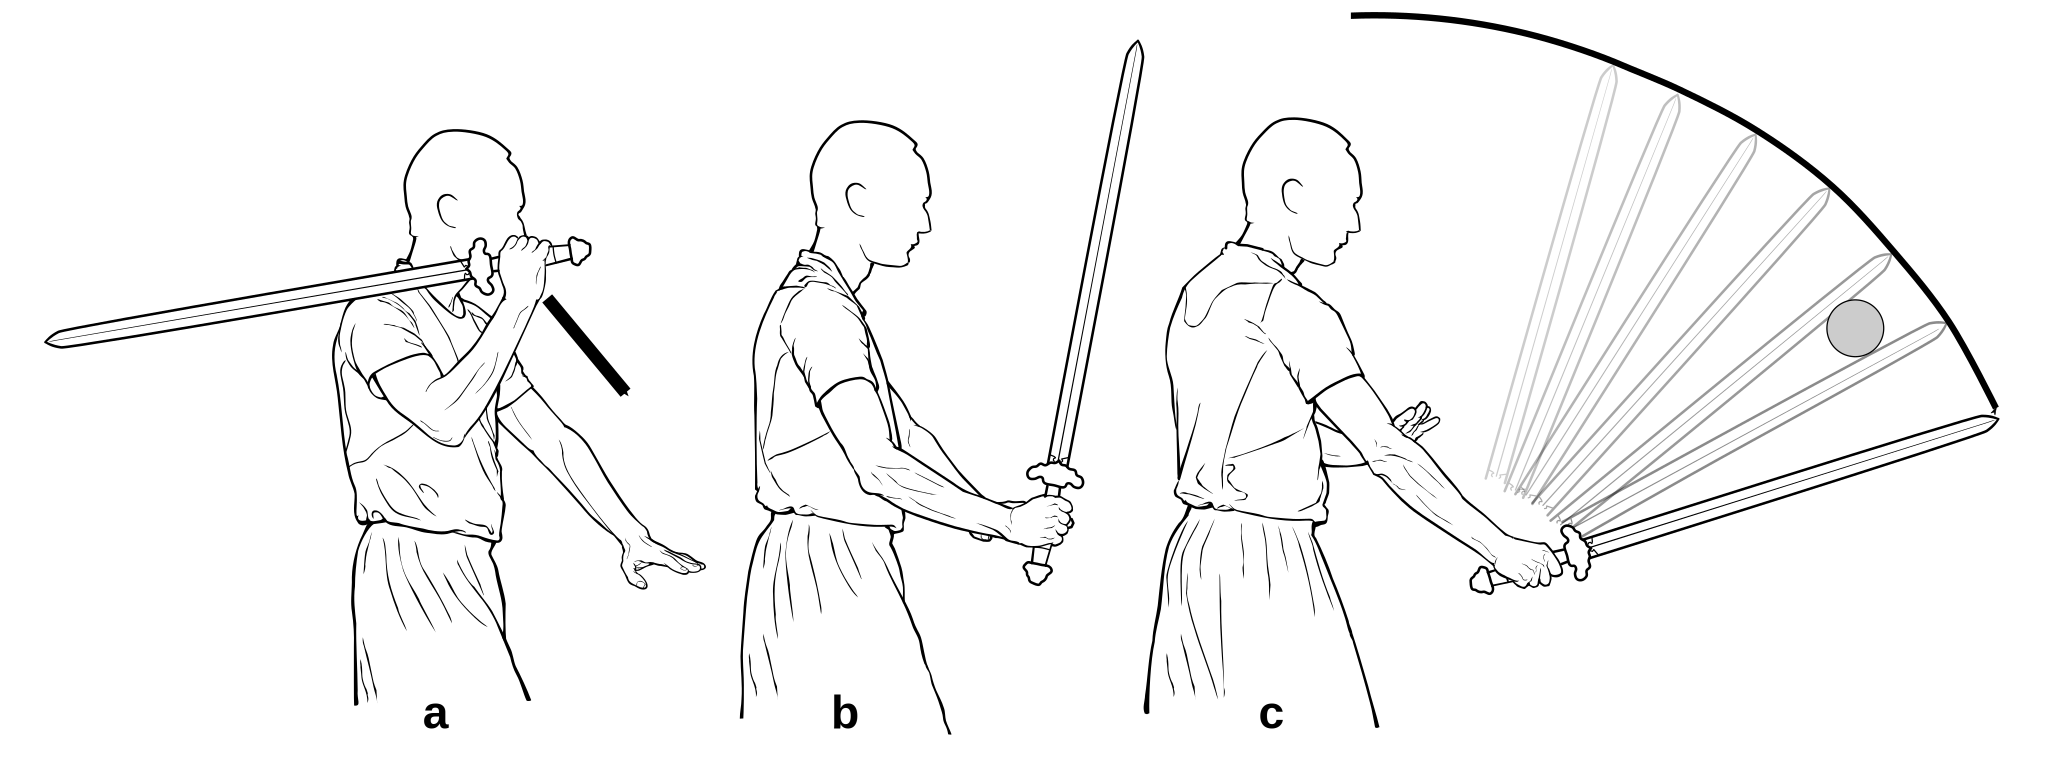
\includegraphics[width=1.00\textwidth]{../../Images/JibenJianfa/Pi/Pi_juxtaposed.pdf}
	\caption[Coupe \Pi{}]{Coupe \Pi{} : (a) Partant d'une position haute de l'épée, la main droite la tire vers le bas pour accélérer la lame; (b) montre la fin de la phase d'accélération, à partir de cet instant, la main n'exercera plus d'action sur la poignée; (c) la main suit la poignée avec juste un contrôle ferme de la trajectoire de l'épée de manière à ce que la lame puisse librement traverser la cible représentée par un cercle gris. Notez que la trajectoire de la pointe n'est pas un cercle mais un arc allongé.}
	\label{fig:pi_cut}
\end{figure}

Il est absolument indispensable que le plat de la lame soit parfaitement aligné avec la trajectoire de la l'épée pour garantir que le poids de la lame soit derrière le tranchant pour le pousser à travers la cible. Si jamais la lame atteignait la cible avec un angle, aussi petit soit-il, elle tendrait à tourner autour de son axe et pourrait rebondir dangereusement au lieu de trancher. Lorsque l'alignement est correct, au contraire, et que la prise est relâchée, la lame pourra traverser la cible de part en part sans retour notable.

Après la coupe, la poignée bute naturellement contre le talon de la main et les doigts resserrent leur prise pour arrêter l'épée dans une position de garde à hauteur de taille, sans aucune tension ni rebond. Grâce à une bonne structure corporelle, l'énergie de l'épée retourne ainsi au corps, aidant le recentrage, et la préparation de la technique suivante.

\section{\Hua}
Le verbe \Hua{} \begin{CJK*}{UTF8}{bsmi}劃\end{CJK*} signifie \textit{délimiter}, \textit{tracer}. Ce caractère est aussi une variante du mot désignant un trait dans un caractère chinois.
La partie de gauche de ce caractère étant la clé du pinceau, ces observation suggèrent que cette technique évoque la notion de calligraphie, d'écriture et de dessin.

Le \Yangjia{} \Michuan{} présente la technique \Hua{} emblématique comme une coupe horizontale ou un large mouvement horizontal dans le but de maintenir les adversaires à distance. L'idée est ici de balayer l'espace avec l'épée pour délimiter la zone la plus large possible autour de soi et d'entailler quiconque ose s'approcher.

D'une manière plus générale, les coupes \Hua{} ne sont pas systématiquement horizontales et s'appliquent à différentes distances, depuis des entailles réalisées à longue distance avec la pointe de l'épée, jusqu'à des coupes glissées avec toute la longueur du tranchant à courte distance. Dans tous les cas, les coupes \Hua{} ont pour caractéristique commune le fait que la lame trace progressivement une longue entaille, au contraire de \Pi{} qui fend la cible d'un coup. 

Pour réaliser une coupe \Hua{} à longue distance, l'épée est lancée en avant et, lorsque le bras a presque atteint son extension complète, juste avant que la lame ne frappe la cible, la prise se resserre doucement sur la poignée pour assurer la connexion entre les centres de l'épée et du corps. La rotation continue ainsi à partir de l'épaule tandis que l'épée tire le corps en avant jusqu'à ce que la portée maximale soit atteinte (fig. \ref{fig:hua_cut} a-c). Ensuite, la prise agissant comme un levier, l'inertie de l'épée repousse la poignée contre le talon de la main, engendrant un mouvement vers l'arrière qui génère une coupe glissée et recentre le corps dans une posture de garde (fig. \ref{fig:hua_cut} d-f). 

\begin{figure}[ht]
\centering
	\includegraphics[width=1.00\textwidth]{../../Images/JibenJianfa/Hua/Hua.pdf}
	\caption[Coupe \Hua{}]{Coupe \Hua{} : (a) \'{A} partir d'une position haute de l'épée, (b) la main droite lance le pommeau vers l'avant; (c) montre la fin de la phase active de la technique; (d) à (f) pendant la phase passive, l'inertie de l'épée repousse la main en arrière, réalisant la coupe glissée et recentrant le corps en position.}
	\label{fig:hua_cut}
\end{figure}

\'{A} plus courte distance, la dynamique des coupes \Hua{} utilise moins l'inertie de l'épée mais s'appuie plus sur la structure et le mouvement du corps. Dès que le tranchant est en contact, la coupe est effectuée en pressant le tranchant contre la cible et en tirant l'épée selon une direction parallèle à l'épée, en se déplaçant ou en tournant le corps. Il est parfois possible, en particulier en passant dans le dos de l'adversaire, de réaliser avec le faux tranchant une coupe \Hua{} à courte distance.

En plus d'être une coupe glissée, \Hua{} peut aussi être utilisé pour maintenir des adversaires à distance ou les obliger à réagir de façon à exploiter leur action et prendre le contrôle du rythme. Pour ce faire, on peut lancer une coupe \Hua{} sans toutefois s'engager totalement, ou faire des moulinets tout en avançant. La distance doit dans ce cas est suffisamment courte pour que ces coupes soient clairement perçues comme une menace bien qu'on puisse être légèrement hors de mesure. La distance idéale est à la limite supérieure de la mesure courte, distance à laquelle, bien qu'elle soit incertaine, une touche est tout à fait plausible et l'adversaire ne peut que se sentir obligé de réagir défensivement. Il est important dans ce cas de se préparer à doubler avec une attaque plus engagée ou un contrôle de la lame selon les circonstances. C'est cette seconde intention qui permettra de prendre l'initiative en exploitant l'action de l'adversaire.

En rompant la distance après une attaque infructueuse, il est possible de maintenir l'adversaire à distance avec une série de moulinets que Maître Wang Yennien décrivait également comme étant des coupes \Hua{}. Cette application de la technique correspond parfaitement à la traduction \textit{délimiter} puisqu'elle crée en effet une zone de sécurité empêchant l'adversaire d'entrer et d'attaquer pendant qu'on se place hors de mesure.


\section{\Ci{}}
On trouve le mot \Ci{} \begin{CJK*}{UTF8}{bsmi}刺\end{CJK*}, signifiant \textit{estoquer}, \textit{percer}, \textit{poignarder}, dans le \WubeiZhi{} comme terme générique désignant l'ensemble des techniques d'estoc à l'épée. D'autres traités anciens le mentionnent aussi pour décrire les estocs avec diverses armes. 

Dans la tradition du \Yangjia{} \Michuan{}, \Ci{} est défini comme un estoc horizontal ou remontant, poussant la pointe puissamment à travers la cible. 

On réalise généralement la technique formelle en commençant sur le pied droit, pied gauche en avant, soit avec une passe avant (\Ci{} long), soit avec un simple transfert de poids sur le pied gauche (\Ci{} court). Dans le contexte formel des exercices et de la forme, la cible du \Ci{} court est l'abdomen, celle du long est la base de la gorge. En assaut par contre, on peut viser d'autres cibles telles que le torse, ou même le visage.

Que la technique réalisée soit longue ou courte, on commence invariablement par créer dans le corps une structure spiralée connectant le pied gauche et l'épée. Dès que la taille bouge, le bras droit pousse sur la poignée et se lève en un mouvement spiralé qui s'achèvera avec une position d'épée horizontale, sur son plat, le pommeau orienté vers la hanche gauche. Dans le même temps, on transfère le poids sur le pied gauche. La prise de l'épée s'adapte progressivement pour maintenir une connexion ininterrompue entre la main et la poignée, sans aucun angle, permettant de pousser sans effort l'épée vers avant. Cet ajustement permet également d'exercer sur la poignée une action oblique atteignant au delà de la garde le point générant un point pivot dans la pointe de la lame pour la stabiliser\footnote{Voyez le chapitre \ref*{ch:epeechinoise} pour de plus amples détails sur les points pivots.}. 


La passe avant du \Ci{} long permet une portée plus longue. Le bras droit doit être étendu avant d'avancer pour augmenter la précision de l'estoc et placer le corps derrière l'épée, aussi loin que possible du danger. Engager la lame de l'adversaire pour la contrôler avec la garde ou le fort de la lame, permet encore une meilleure protection. 

\begin{figure}[ht]
\centering
	\includegraphics[width=1.00\textwidth]{../../Images/JibenJianfa/Ci/Ci_thrust_arc.pdf}
	\caption[Estoc \Ci{} long]{\`{A} la fin de l'estoc \Ci{} long, l'épée est alignée avec la hanche gauche mais sa pointe est dirigée vers le centre, visant la base de la gorge. La puissance de toute la structure du corps se concentre dans l'épée pour pousser la pointe à travers la cible.}
	\label{fig:ci_thrust}
\end{figure}

Idéalement, le talon droit devrait toucher le sol exactement au moment où la pointe de la lame atteint la cible. Le relâchement de la structure achève alors le pas en poussant la lame au travers de la cible. Il est important de ne pas se laisser tomber dans la jambe droite de manière à conserver une capacité de se retirer rapidement en cas de nécessité. Cela ne signifie toutefois pas qu'on ne doit jamais transférer le poids sur la jambe droite, mais que la polarité vide/plein entre les deux jambes doit être maintenue en toutes circonstances pour éviter la double lourdeur. L'arc de force venant du pied gauche, traversant le dos, spiralant le long du bras droit jusqu'à la pointe de l'épée, et soutenu par la spirale du bras gauche, génère ainsi une structure à la fois puissante et mobile.



\section{\Liao}
\Liao{} \begin{CJK*}{UTF8}{bsmi}撩\end{CJK*} est une coupe montante.

\section{\Zha}
\Zha{} \begin{CJK*}{UTF8}{bsmi}扎\end{CJK*} est un coup d'estoc descendant.

\section{\Mo}
\Mo{} \begin{CJK*}{UTF8}{bsmi}抹\end{CJK*} recouvre toutes les techniques de contr\^{o}le du centre de la lame de l'adversaire. 

\section{\Duo}
\Duo{} \begin{CJK*}{UTF8}{bsmi}剁\end{CJK*} est réalisé avec les deux bras étendus, pour un coup de pointe ou de taille puissant.
Combiné avec \Mo{}, \Duo{} peut aussi \^{e}tre utilisé pour dévier l'épée de l'adversaire.

\section{\Tiao}
\Tiao{} \begin{CJK*}{UTF8}{bsmi}挑\end{CJK*} est une coupe rapide réalisée avec le faux tranchant.


\section{\Dian}
\Dian{} \begin{CJK*}{UTF8}{bsmi}點\end{CJK*} est un estoc rapide ou une coupe légère réalisée avec l'extrémité de la lame.